
RF (radio frequency) based positioning problem is concerned with inferring agent/robot position in space from distance measurements to a number of known static or dynamic beacons/landmarks. For instance, in three dimensional case position can be computed by having at least three distance measurements. Technique for doing this is called multilateration.

The chapter is divided in a following way: first describing general methods of measuring distance between two RF devices/antennas, secondly investigating existing protocols making measurements and lastly selecting an algorithm to iteratively compute and track position of a robot over time.

% TODO: put it in a better way : )
Requirements for application:
\begin{itemize}
    \item Ranging max distance - at least 100 meters.
\end{itemize}

\subsection{Range measurement methods}

Literature points out two main methods for making distance measurements over RF antennas: RSSI (Received Signal Strength Indication) and time based methods.
% TODO: AoA?

\subsubsection{RSSI}

As the name suggests the received signal strength hints at the power of incoming radio signal. There is non-linear corelation between RSSI and distance between two antennas \cite{rssi-curves}:
$$
R S S I=-10 n \log _{10}(d)+C
$$
thus it is possible, for instance, to fit a curve on a measured experimental values like shown in \cite{rssi-curves}. However, the main disadvantage that for commercial protocols the quantity over distance curve flattens out at certain distance and further it's impossible to tell the a difference between different measurements. The effect can be seen in Figure \ref{fig:rssi-curves}. Due to this limitation the method is not suitable according to application requirements thus later comparison of available RF technologies for positioning will focus mainly on time based methods.
\begin{figure}
    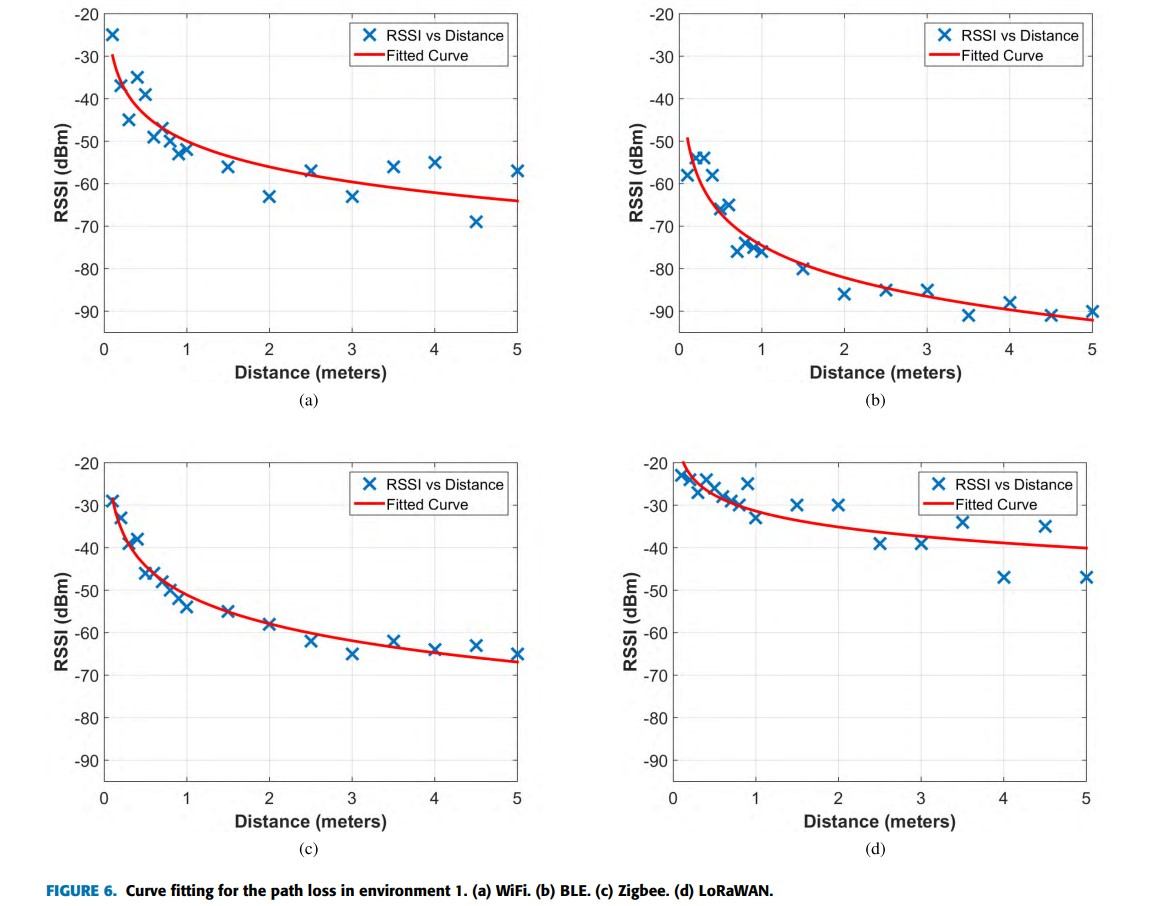
\includegraphics[width=\linewidth]{figures/RSSICurves.jpg}
    \caption{Various protocol RSSI over distance curves \cite{rssi-curves}.}
    \label{fig:rssi-curves}
\end{figure}
  
\subsubsection{Time based}

These methods are based on measuring radio wave propagation time between (or ToF - \emph{Time of Flight}) antennas/devices and calculating the distance by knowing light speed i.e. $d=ct$, where $c=10e-8$ m/s. One obvious drawback here is that two clock must be synchronized if to infer the distance by ToA (\emph{Time of Arrival}). However, this can be avoided by doing a round trip (in literature referred as TDoA - \emph{Time Difference of Arrival}) and relying solely on one clock. The scheme is illustrated in \ref{fig:RTT} where $T_{prop}$ is propagation time in which we are interested in for ranging applications. The value can be computed by $T_{prop} = \frac{1}{2}(T_{round} - T_{reply})$. Also, Figure \ref{fig:RTT} correctly indicates the scale of $T_{round}$ and $T_{prop}$. Important thing to notice here, if the distances we're measuring are in order of meters, $T_{prop} = d/c$ evaluates to nanosecond scale while for response computer might have to execute hundreds of instructions taking up way more time than the time we're interested in. Thus it's of most importance to know how much time computation takes in the responding device. When selecting/designing a system to use RTT for positioning, responding device must have very fine granularity control of computing resources. If one would try to make these computations on OS (Operating system) level, the time jitter introduced by OS scheduling system would be so large that propagation time would vanish in the error of $T_{reply}$ measurement.
\begin{figure}[H]
    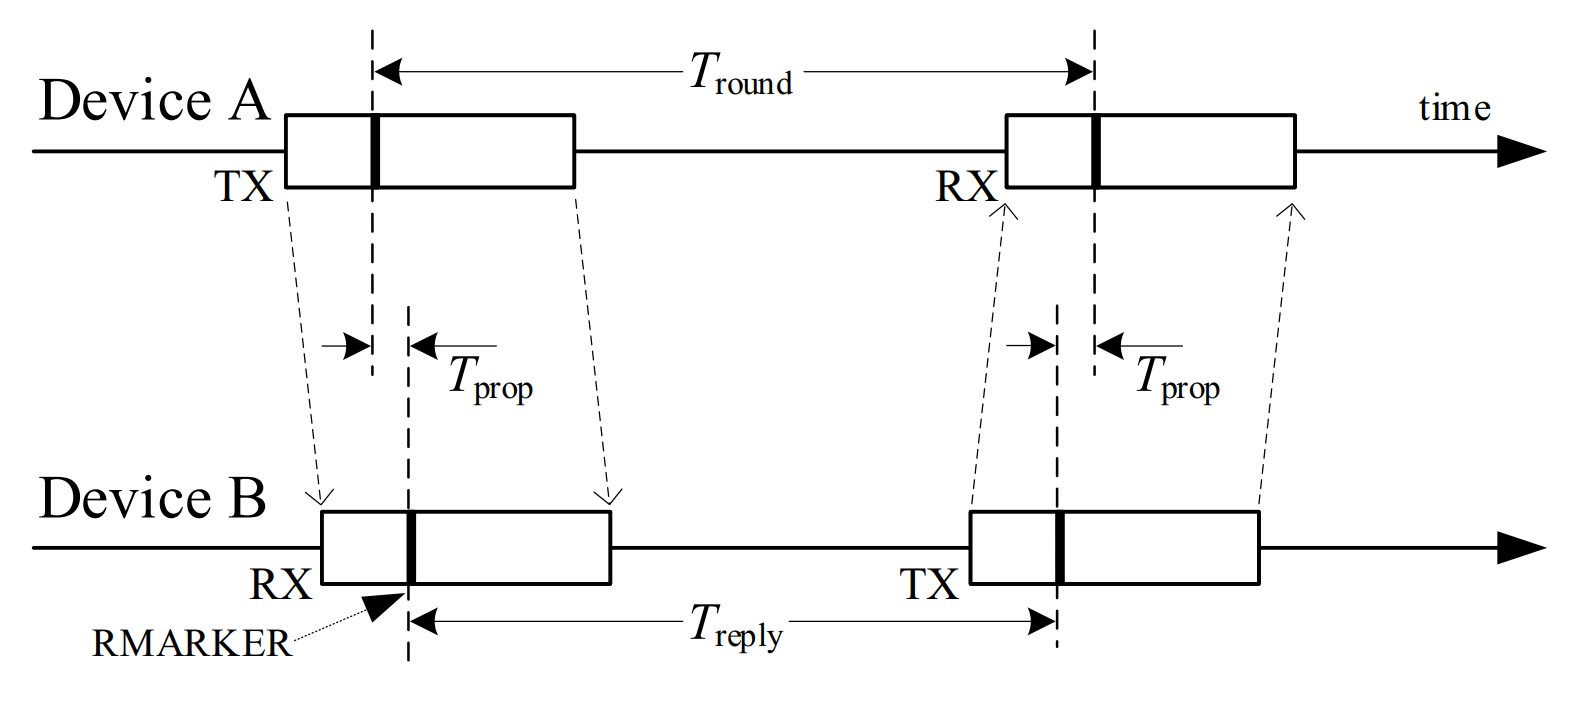
\includegraphics[width=\linewidth]{figures/RTT.jpg}
    \caption{Round trip time \cite{9179124}.}
    \label{fig:RTT}
\end{figure}
  
\subsection{RF positioning}

There are many existing protocols/technologies to exchange data between devices over the air i.e. by transmitting it over electromagnetic waves. In this chapterF, a few of most popular ones will be reviewed in terms of how suitable each of them is for positioning applications. Namely, paper investigates WiFi, UWB (Ultra Wide Band) and BLE (Bluetooth Low Energy) protocols.

\subsubsection{WiFi}

FTM RTT: RTT could be obtained by FTM protocol but is difficult to obtain bc hardware support is very limited. Even then requires quite a bit of effort to install required driver, firmware, kernel version. The distance measurement is not that precise. Best case scenario gives 1-2m accuracy which is nice but more crude estimation would also work.
% https://www.banshee-navigation.eu/blog/posts/what_is_wi-fi_rtt
% https://www.winlab.rutgers.edu/~gruteser/projects/ftm/Setups.htm

Positioning base on WiFi signal strength is way easier. Basically could be implemented with any WiFi card without spending additional time on setup. Accuracy is worse ~10m. But meets the requirements and prob is worth trying first before going to alternatives. Turns out that the distance to signal curve flattens out at around 20m and cannot measure distances beyond that...
% TODO:

So wifi frequency is max 80MHz which in time based methods alone results in max theoretical distance resolution of 3.5m of time based methods.

% TODO:
% Measuring Round Trip Times to Determine the Distance Between WLAN Nodes 803 pdf page; data collection & processing https://link.springer.com/content/pdf/10.1007/b136094.pdf
% The resolution of these hardware time stamps, which are implemented in most current WLAN products, is 1 μs corresponding to 300 m. :D and they  don't say how they get those hardware timestamps either, mistery still.

% TODO:
% why some papers say that distance resolution is dependant on bandwidth? even though the wifi freq is 2.4 of 5 GHz. How come the distance resolution calculation only takes in bandwidth for example 20MHz or 40MHz???
% https://github.com/domienschepers/wifi-ftm

\subsubsection{BLE}

Easily available but no support for precision time stamping...

\subsubsection{UWB}

How does UWB solve time stamping? THis is very well defined in the official standard 802154z-2020, read the pdf and do a summary.
% https://www.mouser.dk/ProductDetail/Qorvo/DWM3000EVB?qs=iLbezkQI%252BsgO%252Bhh8kPU5Xg%3D%3D
% https://www.mouser.dk/new/qorvo/qorvo-dws3000evb-arduino-shield/
% https://github.com/Makerfabs/Makerfabs-ESP32-UWB
% https://arxiv.org/pdf/2202.02190.pdf check this out too, An Overview of UWB Standards

\subsection{Position from distance measurement}

However, solution (from 3 beacons) is not unique and adding fourth one allows to come up with a distinctive robot position easier.